% Created by tikzDevice version 0.12.3.1 on 2022-09-05 08:11:26
% !TEX encoding = UTF-8 Unicode
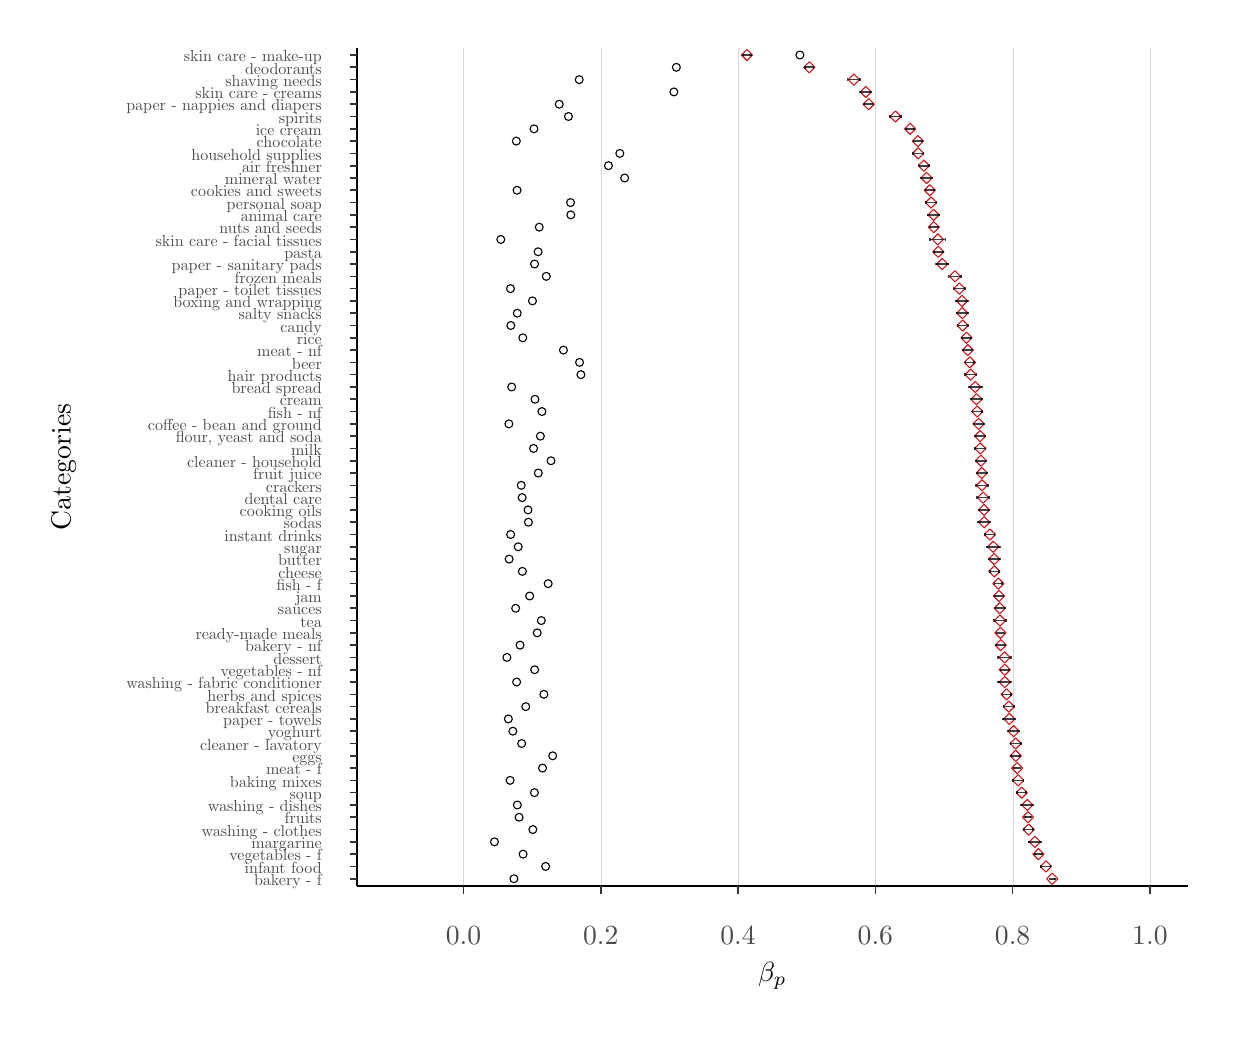
\begin{tikzpicture}[x=1pt,y=1pt]
\definecolor{fillColor}{RGB}{255,255,255}
\path[use as bounding box,fill=fillColor,fill opacity=0.00] (0,0) rectangle (433.62,361.35);
\begin{scope}
\path[clip] (  0.00,  0.00) rectangle (433.62,361.35);
\definecolor{drawColor}{RGB}{255,255,255}
\definecolor{fillColor}{RGB}{255,255,255}

\path[draw=drawColor,line width= 0.6pt,line join=round,line cap=round,fill=fillColor] (  0.00,  0.00) rectangle (433.62,361.35);
\end{scope}
\begin{scope}
\path[clip] (119.04, 51.15) rectangle (419.17,354.12);
\definecolor{drawColor}{RGB}{255,255,255}

\path[draw=drawColor,line width= 0.3pt,line join=round] (132.68, 51.15) --
	(132.68,354.12);

\path[draw=drawColor,line width= 0.3pt,line join=round] (182.29, 51.15) --
	(182.29,354.12);

\path[draw=drawColor,line width= 0.3pt,line join=round] (231.90, 51.15) --
	(231.90,354.12);

\path[draw=drawColor,line width= 0.3pt,line join=round] (281.51, 51.15) --
	(281.51,354.12);

\path[draw=drawColor,line width= 0.3pt,line join=round] (331.11, 51.15) --
	(331.11,354.12);

\path[draw=drawColor,line width= 0.3pt,line join=round] (380.72, 51.15) --
	(380.72,354.12);
\definecolor{drawColor}{gray}{0.85}

\path[draw=drawColor,line width= 0.1pt,line join=round] (157.49, 51.15) --
	(157.49,354.12);

\path[draw=drawColor,line width= 0.1pt,line join=round] (207.09, 51.15) --
	(207.09,354.12);

\path[draw=drawColor,line width= 0.1pt,line join=round] (256.70, 51.15) --
	(256.70,354.12);

\path[draw=drawColor,line width= 0.1pt,line join=round] (306.31, 51.15) --
	(306.31,354.12);

\path[draw=drawColor,line width= 0.1pt,line join=round] (355.92, 51.15) --
	(355.92,354.12);

\path[draw=drawColor,line width= 0.1pt,line join=round] (405.52, 51.15) --
	(405.52,354.12);
\definecolor{drawColor}{RGB}{0,0,0}

\path[draw=drawColor,line width= 0.4pt,line join=round,line cap=round] (209.86,311.48) circle (  1.43);

\path[draw=drawColor,line width= 0.4pt,line join=round,line cap=round] (196.26,293.71) circle (  1.43);

\path[draw=drawColor,line width= 0.4pt,line join=round,line cap=round] (175.71, 53.82) circle (  1.43);

\path[draw=drawColor,line width= 0.4pt,line join=round,line cap=round] (177.92,138.22) circle (  1.43);

\path[draw=drawColor,line width= 0.4pt,line join=round,line cap=round] (174.31, 89.36) circle (  1.43);

\path[draw=drawColor,line width= 0.4pt,line join=round,line cap=round] (199.42,240.40) circle (  1.43);

\path[draw=drawColor,line width= 0.4pt,line join=round,line cap=round] (182.40,262.61) circle (  1.43);

\path[draw=drawColor,line width= 0.4pt,line join=round,line cap=round] (174.89,231.51) circle (  1.43);

\path[draw=drawColor,line width= 0.4pt,line join=round,line cap=round] (179.98,116.01) circle (  1.43);

\path[draw=drawColor,line width= 0.4pt,line join=round,line cap=round] (173.98,169.32) circle (  1.43);

\path[draw=drawColor,line width= 0.4pt,line join=round,line cap=round] (174.58,253.73) circle (  1.43);

\path[draw=drawColor,line width= 0.4pt,line join=round,line cap=round] (178.76,164.88) circle (  1.43);

\path[draw=drawColor,line width= 0.4pt,line join=round,line cap=round] (176.57,320.36) circle (  1.43);

\path[draw=drawColor,line width= 0.4pt,line join=round,line cap=round] (189.10,204.86) circle (  1.43);

\path[draw=drawColor,line width= 0.4pt,line join=round,line cap=round] (178.50,102.69) circle (  1.43);

\path[draw=drawColor,line width= 0.4pt,line join=round,line cap=round] (173.89,218.19) circle (  1.43);

\path[draw=drawColor,line width= 0.4pt,line join=round,line cap=round] (176.84,302.59) circle (  1.43);

\path[draw=drawColor,line width= 0.4pt,line join=round,line cap=round] (180.79,187.09) circle (  1.43);

\path[draw=drawColor,line width= 0.4pt,line join=round,line cap=round] (178.36,195.97) circle (  1.43);

\path[draw=drawColor,line width= 0.4pt,line join=round,line cap=round] (183.31,227.07) circle (  1.43);

\path[draw=drawColor,line width= 0.4pt,line join=round,line cap=round] (178.67,191.53) circle (  1.43);

\path[draw=drawColor,line width= 0.4pt,line join=round,line cap=round] (234.40,347.02) circle (  1.43);

\path[draw=drawColor,line width= 0.4pt,line join=round,line cap=round] (173.16,133.78) circle (  1.43);

\path[draw=drawColor,line width= 0.4pt,line join=round,line cap=round] (189.72, 98.24) circle (  1.43);

\path[draw=drawColor,line width= 0.4pt,line join=round,line cap=round] (188.09,160.44) circle (  1.43);

\path[draw=drawColor,line width= 0.4pt,line join=round,line cap=round] (185.83,222.63) circle (  1.43);

\path[draw=drawColor,line width= 0.4pt,line join=round,line cap=round] (185.26,213.74) circle (  1.43);

\path[draw=drawColor,line width= 0.4pt,line join=round,line cap=round] (187.40,271.49) circle (  1.43);

\path[draw=drawColor,line width= 0.4pt,line join=round,line cap=round] (184.51,200.42) circle (  1.43);

\path[draw=drawColor,line width= 0.4pt,line join=round,line cap=round] (177.56, 76.03) circle (  1.43);

\path[draw=drawColor,line width= 0.4pt,line join=round,line cap=round] (199.91,235.96) circle (  1.43);

\path[draw=drawColor,line width= 0.4pt,line join=round,line cap=round] (186.53,120.45) circle (  1.43);

\path[draw=drawColor,line width= 0.4pt,line join=round,line cap=round] (213.97,315.92) circle (  1.43);

\path[draw=drawColor,line width= 0.4pt,line join=round,line cap=round] (182.96,324.80) circle (  1.43);

\path[draw=drawColor,line width= 0.4pt,line join=round,line cap=round] (187.16, 58.26) circle (  1.43);

\path[draw=drawColor,line width= 0.4pt,line join=round,line cap=round] (174.52,178.21) circle (  1.43);

\path[draw=drawColor,line width= 0.4pt,line join=round,line cap=round] (181.40,155.99) circle (  1.43);

\path[draw=drawColor,line width= 0.4pt,line join=round,line cap=round] (168.67, 67.15) circle (  1.43);

\path[draw=drawColor,line width= 0.4pt,line join=round,line cap=round] (186.04, 93.80) circle (  1.43);

\path[draw=drawColor,line width= 0.4pt,line join=round,line cap=round] (193.59,244.84) circle (  1.43);

\path[draw=drawColor,line width= 0.4pt,line join=round,line cap=round] (182.79,209.30) circle (  1.43);

\path[draw=drawColor,line width= 0.4pt,line join=round,line cap=round] (215.72,307.03) circle (  1.43);

\path[draw=drawColor,line width= 0.4pt,line join=round,line cap=round] (184.86,289.26) circle (  1.43);

\path[draw=drawColor,line width= 0.4pt,line join=round,line cap=round] (192.08,333.69) circle (  1.43);

\path[draw=drawColor,line width= 0.4pt,line join=round,line cap=round] (183.16,275.94) circle (  1.43);

\path[draw=drawColor,line width= 0.4pt,line join=round,line cap=round] (174.46,267.05) circle (  1.43);

\path[draw=drawColor,line width= 0.4pt,line join=round,line cap=round] (173.69,111.57) circle (  1.43);

\path[draw=drawColor,line width= 0.4pt,line join=round,line cap=round] (184.44,280.38) circle (  1.43);

\path[draw=drawColor,line width= 0.4pt,line join=round,line cap=round] (196.16,298.15) circle (  1.43);

\path[draw=drawColor,line width= 0.4pt,line join=round,line cap=round] (184.12,142.67) circle (  1.43);

\path[draw=drawColor,line width= 0.4pt,line join=round,line cap=round] (178.91,249.28) circle (  1.43);

\path[draw=drawColor,line width= 0.4pt,line join=round,line cap=round] (176.91,258.17) circle (  1.43);

\path[draw=drawColor,line width= 0.4pt,line join=round,line cap=round] (176.34,151.55) circle (  1.43);

\path[draw=drawColor,line width= 0.4pt,line join=round,line cap=round] (199.29,342.57) circle (  1.43);

\path[draw=drawColor,line width= 0.4pt,line join=round,line cap=round] (233.51,338.13) circle (  1.43);

\path[draw=drawColor,line width= 0.4pt,line join=round,line cap=round] (170.96,284.82) circle (  1.43);

\path[draw=drawColor,line width= 0.4pt,line join=round,line cap=round] (279.04,351.46) circle (  1.43);

\path[draw=drawColor,line width= 0.4pt,line join=round,line cap=round] (180.94,182.65) circle (  1.43);

\path[draw=drawColor,line width= 0.4pt,line join=round,line cap=round] (183.12, 84.92) circle (  1.43);

\path[draw=drawColor,line width= 0.4pt,line join=round,line cap=round] (195.42,329.25) circle (  1.43);

\path[draw=drawColor,line width= 0.4pt,line join=round,line cap=round] (177.24,173.76) circle (  1.43);

\path[draw=drawColor,line width= 0.4pt,line join=round,line cap=round] (185.59,147.11) circle (  1.43);

\path[draw=drawColor,line width= 0.4pt,line join=round,line cap=round] (179.01, 62.70) circle (  1.43);

\path[draw=drawColor,line width= 0.4pt,line join=round,line cap=round] (183.20,129.34) circle (  1.43);

\path[draw=drawColor,line width= 0.4pt,line join=round,line cap=round] (182.54, 71.59) circle (  1.43);

\path[draw=drawColor,line width= 0.4pt,line join=round,line cap=round] (176.94, 80.47) circle (  1.43);

\path[draw=drawColor,line width= 0.4pt,line join=round,line cap=round] (176.68,124.90) circle (  1.43);

\path[draw=drawColor,line width= 0.4pt,line join=round,line cap=round] (175.32,107.13) circle (  1.43);
\definecolor{drawColor}{RGB}{203,24,29}

\path[draw=drawColor,line width= 0.4pt,line join=round,line cap=round] (321.80,311.48) --
	(323.82,313.49) --
	(325.84,311.48) --
	(323.82,309.46) --
	cycle;

\path[draw=drawColor,line width= 0.4pt,line join=round,line cap=round] (325.32,293.71) --
	(327.33,295.72) --
	(329.35,293.71) --
	(327.33,291.69) --
	cycle;

\path[draw=drawColor,line width= 0.4pt,line join=round,line cap=round] (368.21, 53.82) --
	(370.23, 55.84) --
	(372.25, 53.82) --
	(370.23, 51.80) --
	cycle;

\path[draw=drawColor,line width= 0.4pt,line join=round,line cap=round] (349.60,138.22) --
	(351.61,140.24) --
	(353.63,138.22) --
	(351.61,136.21) --
	cycle;

\path[draw=drawColor,line width= 0.4pt,line join=round,line cap=round] (355.88, 89.36) --
	(357.90, 91.38) --
	(359.91, 89.36) --
	(357.90, 87.34) --
	cycle;

\path[draw=drawColor,line width= 0.4pt,line join=round,line cap=round] (338.41,240.40) --
	(340.43,242.42) --
	(342.45,240.40) --
	(340.43,238.38) --
	cycle;

\path[draw=drawColor,line width= 0.4pt,line join=round,line cap=round] (335.59,262.61) --
	(337.60,264.63) --
	(339.62,262.61) --
	(337.60,260.59) --
	cycle;

\path[draw=drawColor,line width= 0.4pt,line join=round,line cap=round] (340.39,231.51) --
	(342.41,233.53) --
	(344.43,231.51) --
	(342.41,229.50) --
	cycle;

\path[draw=drawColor,line width= 0.4pt,line join=round,line cap=round] (352.49,116.01) --
	(354.51,118.03) --
	(356.53,116.01) --
	(354.51,113.99) --
	cycle;

\path[draw=drawColor,line width= 0.4pt,line join=round,line cap=round] (347.23,169.32) --
	(349.25,171.34) --
	(351.27,169.32) --
	(349.25,167.30) --
	cycle;

\path[draw=drawColor,line width= 0.4pt,line join=round,line cap=round] (335.83,253.73) --
	(337.85,255.74) --
	(339.87,253.73) --
	(337.85,251.71) --
	cycle;

\path[draw=drawColor,line width= 0.4pt,line join=round,line cap=round] (347.27,164.88) --
	(349.29,166.90) --
	(351.31,164.88) --
	(349.29,162.86) --
	cycle;

\path[draw=drawColor,line width= 0.4pt,line join=round,line cap=round] (319.65,320.36) --
	(321.67,322.38) --
	(323.68,320.36) --
	(321.67,318.34) --
	cycle;

\path[draw=drawColor,line width= 0.4pt,line join=round,line cap=round] (342.48,204.86) --
	(344.50,206.88) --
	(346.51,204.86) --
	(344.50,202.84) --
	cycle;

\path[draw=drawColor,line width= 0.4pt,line join=round,line cap=round] (355.00,102.69) --
	(357.01,104.70) --
	(359.03,102.69) --
	(357.01,100.67) --
	cycle;

\path[draw=drawColor,line width= 0.4pt,line join=round,line cap=round] (341.61,218.19) --
	(343.63,220.20) --
	(345.65,218.19) --
	(343.63,216.17) --
	cycle;

\path[draw=drawColor,line width= 0.4pt,line join=round,line cap=round] (323.97,302.59) --
	(325.99,304.61) --
	(328.01,302.59) --
	(325.99,300.57) --
	cycle;

\path[draw=drawColor,line width= 0.4pt,line join=round,line cap=round] (343.59,187.09) --
	(345.60,189.11) --
	(347.62,187.09) --
	(345.60,185.07) --
	cycle;

\path[draw=drawColor,line width= 0.4pt,line join=round,line cap=round] (342.82,195.97) --
	(344.83,197.99) --
	(346.85,195.97) --
	(344.83,193.96) --
	cycle;

\path[draw=drawColor,line width= 0.4pt,line join=round,line cap=round] (340.84,227.07) --
	(342.86,229.09) --
	(344.87,227.07) --
	(342.86,225.05) --
	cycle;

\path[draw=drawColor,line width= 0.4pt,line join=round,line cap=round] (343.21,191.53) --
	(345.23,193.55) --
	(347.25,191.53) --
	(345.23,189.51) --
	cycle;

\path[draw=drawColor,line width= 0.4pt,line join=round,line cap=round] (280.42,347.02) --
	(282.44,349.03) --
	(284.45,347.02) --
	(282.44,345.00) --
	cycle;

\path[draw=drawColor,line width= 0.4pt,line join=round,line cap=round] (350.98,133.78) --
	(353.00,135.80) --
	(355.01,133.78) --
	(353.00,131.76) --
	cycle;

\path[draw=drawColor,line width= 0.4pt,line join=round,line cap=round] (355.00, 98.24) --
	(357.02,100.26) --
	(359.03, 98.24) --
	(357.02, 96.23) --
	cycle;

\path[draw=drawColor,line width= 0.4pt,line join=round,line cap=round] (348.73,160.44) --
	(350.75,162.45) --
	(352.77,160.44) --
	(350.75,158.42) --
	cycle;

\path[draw=drawColor,line width= 0.4pt,line join=round,line cap=round] (341.09,222.63) --
	(343.11,224.65) --
	(345.12,222.63) --
	(343.11,220.61) --
	cycle;

\path[draw=drawColor,line width= 0.4pt,line join=round,line cap=round] (342.16,213.74) --
	(344.18,215.76) --
	(346.19,213.74) --
	(344.18,211.73) --
	cycle;

\path[draw=drawColor,line width= 0.4pt,line join=round,line cap=round] (333.05,271.49) --
	(335.07,273.51) --
	(337.09,271.49) --
	(335.07,269.48) --
	cycle;

\path[draw=drawColor,line width= 0.4pt,line join=round,line cap=round] (342.75,200.42) --
	(344.77,202.43) --
	(346.78,200.42) --
	(344.77,198.40) --
	cycle;

\path[draw=drawColor,line width= 0.4pt,line join=round,line cap=round] (359.46, 76.03) --
	(361.48, 78.05) --
	(363.50, 76.03) --
	(361.48, 74.01) --
	cycle;

\path[draw=drawColor,line width= 0.4pt,line join=round,line cap=round] (338.73,235.96) --
	(340.75,237.97) --
	(342.76,235.96) --
	(340.75,233.94) --
	cycle;

\path[draw=drawColor,line width= 0.4pt,line join=round,line cap=round] (351.74,120.45) --
	(353.76,122.47) --
	(355.78,120.45) --
	(353.76,118.44) --
	cycle;

\path[draw=drawColor,line width= 0.4pt,line join=round,line cap=round] (319.78,315.92) --
	(321.80,317.94) --
	(323.82,315.92) --
	(321.80,313.90) --
	cycle;

\path[draw=drawColor,line width= 0.4pt,line join=round,line cap=round] (316.85,324.80) --
	(318.86,326.82) --
	(320.88,324.80) --
	(318.86,322.79) --
	cycle;

\path[draw=drawColor,line width= 0.4pt,line join=round,line cap=round] (365.93, 58.26) --
	(367.95, 60.28) --
	(369.96, 58.26) --
	(367.95, 56.24) --
	cycle;

\path[draw=drawColor,line width= 0.4pt,line join=round,line cap=round] (345.69,178.21) --
	(347.71,180.22) --
	(349.73,178.21) --
	(347.71,176.19) --
	cycle;

\path[draw=drawColor,line width= 0.4pt,line join=round,line cap=round] (348.98,155.99) --
	(351.00,158.01) --
	(353.02,155.99) --
	(351.00,153.98) --
	cycle;

\path[draw=drawColor,line width= 0.4pt,line join=round,line cap=round] (361.93, 67.15) --
	(363.94, 69.16) --
	(365.96, 67.15) --
	(363.94, 65.13) --
	cycle;

\path[draw=drawColor,line width= 0.4pt,line join=round,line cap=round] (355.54, 93.80) --
	(357.55, 95.82) --
	(359.57, 93.80) --
	(357.55, 91.78) --
	cycle;

\path[draw=drawColor,line width= 0.4pt,line join=round,line cap=round] (337.69,244.84) --
	(339.70,246.86) --
	(341.72,244.84) --
	(339.70,242.82) --
	cycle;

\path[draw=drawColor,line width= 0.4pt,line join=round,line cap=round] (342.22,209.30) --
	(344.24,211.32) --
	(346.25,209.30) --
	(344.24,207.28) --
	cycle;

\path[draw=drawColor,line width= 0.4pt,line join=round,line cap=round] (322.78,307.03) --
	(324.80,309.05) --
	(326.82,307.03) --
	(324.80,305.02) --
	cycle;

\path[draw=drawColor,line width= 0.4pt,line join=round,line cap=round] (325.40,289.26) --
	(327.42,291.28) --
	(329.44,289.26) --
	(327.42,287.25) --
	cycle;

\path[draw=drawColor,line width= 0.4pt,line join=round,line cap=round] (301.89,333.69) --
	(303.91,335.71) --
	(305.93,333.69) --
	(303.91,331.67) --
	cycle;

\path[draw=drawColor,line width= 0.4pt,line join=round,line cap=round] (328.47,275.94) --
	(330.49,277.95) --
	(332.50,275.94) --
	(330.49,273.92) --
	cycle;

\path[draw=drawColor,line width= 0.4pt,line join=round,line cap=round] (334.65,267.05) --
	(336.67,269.07) --
	(338.69,267.05) --
	(336.67,265.04) --
	cycle;

\path[draw=drawColor,line width= 0.4pt,line join=round,line cap=round] (352.69,111.57) --
	(354.71,113.59) --
	(356.73,111.57) --
	(354.71,109.55) --
	cycle;

\path[draw=drawColor,line width= 0.4pt,line join=round,line cap=round] (327.02,280.38) --
	(329.04,282.40) --
	(331.06,280.38) --
	(329.04,278.36) --
	cycle;

\path[draw=drawColor,line width= 0.4pt,line join=round,line cap=round] (324.40,298.15) --
	(326.42,300.17) --
	(328.44,298.15) --
	(326.42,296.13) --
	cycle;

\path[draw=drawColor,line width= 0.4pt,line join=round,line cap=round] (349.48,142.67) --
	(351.50,144.68) --
	(353.52,142.67) --
	(351.50,140.65) --
	cycle;

\path[draw=drawColor,line width= 0.4pt,line join=round,line cap=round] (337.22,249.28) --
	(339.24,251.30) --
	(341.26,249.28) --
	(339.24,247.27) --
	cycle;

\path[draw=drawColor,line width= 0.4pt,line join=round,line cap=round] (335.72,258.17) --
	(337.74,260.19) --
	(339.76,258.17) --
	(337.74,256.15) --
	cycle;

\path[draw=drawColor,line width= 0.4pt,line join=round,line cap=round] (349.27,151.55) --
	(351.29,153.57) --
	(353.30,151.55) --
	(351.29,149.53) --
	cycle;

\path[draw=drawColor,line width= 0.4pt,line join=round,line cap=round] (296.53,342.57) --
	(298.55,344.59) --
	(300.57,342.57) --
	(298.55,340.56) --
	cycle;

\path[draw=drawColor,line width= 0.4pt,line join=round,line cap=round] (300.82,338.13) --
	(302.84,340.15) --
	(304.85,338.13) --
	(302.84,336.11) --
	cycle;

\path[draw=drawColor,line width= 0.4pt,line join=round,line cap=round] (326.89,284.82) --
	(328.90,286.84) --
	(330.92,284.82) --
	(328.90,282.80) --
	cycle;

\path[draw=drawColor,line width= 0.4pt,line join=round,line cap=round] (257.85,351.46) --
	(259.87,353.48) --
	(261.89,351.46) --
	(259.87,349.44) --
	cycle;

\path[draw=drawColor,line width= 0.4pt,line join=round,line cap=round] (343.61,182.65) --
	(345.63,184.67) --
	(347.65,182.65) --
	(345.63,180.63) --
	cycle;

\path[draw=drawColor,line width= 0.4pt,line join=round,line cap=round] (357.18, 84.92) --
	(359.20, 86.93) --
	(361.22, 84.92) --
	(359.20, 82.90) --
	cycle;

\path[draw=drawColor,line width= 0.4pt,line join=round,line cap=round] (311.54,329.25) --
	(313.55,331.26) --
	(315.57,329.25) --
	(313.55,327.23) --
	cycle;

\path[draw=drawColor,line width= 0.4pt,line join=round,line cap=round] (346.90,173.76) --
	(348.92,175.78) --
	(350.93,173.76) --
	(348.92,171.75) --
	cycle;

\path[draw=drawColor,line width= 0.4pt,line join=round,line cap=round] (349.32,147.11) --
	(351.33,149.13) --
	(353.35,147.11) --
	(351.33,145.09) --
	cycle;

\path[draw=drawColor,line width= 0.4pt,line join=round,line cap=round] (363.23, 62.70) --
	(365.24, 64.72) --
	(367.26, 62.70) --
	(365.24, 60.69) --
	cycle;

\path[draw=drawColor,line width= 0.4pt,line join=round,line cap=round] (351.03,129.34) --
	(353.04,131.36) --
	(355.06,129.34) --
	(353.04,127.32) --
	cycle;

\path[draw=drawColor,line width= 0.4pt,line join=round,line cap=round] (359.70, 71.59) --
	(361.71, 73.61) --
	(363.73, 71.59) --
	(361.71, 69.57) --
	cycle;

\path[draw=drawColor,line width= 0.4pt,line join=round,line cap=round] (359.21, 80.47) --
	(361.23, 82.49) --
	(363.24, 80.47) --
	(361.23, 78.46) --
	cycle;

\path[draw=drawColor,line width= 0.4pt,line join=round,line cap=round] (351.04,124.90) --
	(353.06,126.91) --
	(355.08,124.90) --
	(353.06,122.88) --
	cycle;

\path[draw=drawColor,line width= 0.4pt,line join=round,line cap=round] (354.25,107.13) --
	(356.27,109.14) --
	(358.29,107.13) --
	(356.27,105.11) --
	cycle;
\definecolor{drawColor}{RGB}{0,0,0}

\path[draw=drawColor,draw opacity=0.75,line width= 0.6pt,line join=round] (325.70,311.03) --
	(325.70,311.92);

\path[draw=drawColor,draw opacity=0.75,line width= 0.6pt,line join=round] (325.70,311.48) --
	(321.94,311.48);

\path[draw=drawColor,draw opacity=0.75,line width= 0.6pt,line join=round] (321.94,311.03) --
	(321.94,311.92);

\path[draw=drawColor,draw opacity=0.75,line width= 0.6pt,line join=round] (329.53,293.26) --
	(329.53,294.15);

\path[draw=drawColor,draw opacity=0.75,line width= 0.6pt,line join=round] (329.53,293.71) --
	(325.14,293.71);

\path[draw=drawColor,draw opacity=0.75,line width= 0.6pt,line join=round] (325.14,293.26) --
	(325.14,294.15);

\path[draw=drawColor,draw opacity=0.75,line width= 0.6pt,line join=round] (371.21, 53.37) --
	(371.21, 54.26);

\path[draw=drawColor,draw opacity=0.75,line width= 0.6pt,line join=round] (371.21, 53.82) --
	(369.24, 53.82);

\path[draw=drawColor,draw opacity=0.75,line width= 0.6pt,line join=round] (369.24, 53.37) --
	(369.24, 54.26);

\path[draw=drawColor,draw opacity=0.75,line width= 0.6pt,line join=round] (353.38,137.78) --
	(353.38,138.67);

\path[draw=drawColor,draw opacity=0.75,line width= 0.6pt,line join=round] (353.38,138.22) --
	(349.84,138.22);

\path[draw=drawColor,draw opacity=0.75,line width= 0.6pt,line join=round] (349.84,137.78) --
	(349.84,138.67);

\path[draw=drawColor,draw opacity=0.75,line width= 0.6pt,line join=round] (359.82, 88.91) --
	(359.82, 89.80);

\path[draw=drawColor,draw opacity=0.75,line width= 0.6pt,line join=round] (359.82, 89.36) --
	(355.97, 89.36);

\path[draw=drawColor,draw opacity=0.75,line width= 0.6pt,line join=round] (355.97, 88.91) --
	(355.97, 89.80);

\path[draw=drawColor,draw opacity=0.75,line width= 0.6pt,line join=round] (342.00,239.95) --
	(342.00,240.84);

\path[draw=drawColor,draw opacity=0.75,line width= 0.6pt,line join=round] (342.00,240.40) --
	(338.85,240.40);

\path[draw=drawColor,draw opacity=0.75,line width= 0.6pt,line join=round] (338.85,239.95) --
	(338.85,240.84);

\path[draw=drawColor,draw opacity=0.75,line width= 0.6pt,line join=round] (339.73,262.17) --
	(339.73,263.05);

\path[draw=drawColor,draw opacity=0.75,line width= 0.6pt,line join=round] (339.73,262.61) --
	(335.48,262.61);

\path[draw=drawColor,draw opacity=0.75,line width= 0.6pt,line join=round] (335.48,262.17) --
	(335.48,263.05);

\path[draw=drawColor,draw opacity=0.75,line width= 0.6pt,line join=round] (344.75,231.07) --
	(344.75,231.96);

\path[draw=drawColor,draw opacity=0.75,line width= 0.6pt,line join=round] (344.75,231.51) --
	(340.07,231.51);

\path[draw=drawColor,draw opacity=0.75,line width= 0.6pt,line join=round] (340.07,231.07) --
	(340.07,231.96);

\path[draw=drawColor,draw opacity=0.75,line width= 0.6pt,line join=round] (356.46,115.57) --
	(356.46,116.46);

\path[draw=drawColor,draw opacity=0.75,line width= 0.6pt,line join=round] (356.46,116.01) --
	(352.56,116.01);

\path[draw=drawColor,draw opacity=0.75,line width= 0.6pt,line join=round] (352.56,115.57) --
	(352.56,116.46);

\path[draw=drawColor,draw opacity=0.75,line width= 0.6pt,line join=round] (351.28,168.88) --
	(351.28,169.76);

\path[draw=drawColor,draw opacity=0.75,line width= 0.6pt,line join=round] (351.28,169.32) --
	(347.22,169.32);

\path[draw=drawColor,draw opacity=0.75,line width= 0.6pt,line join=round] (347.22,168.88) --
	(347.22,169.76);

\path[draw=drawColor,draw opacity=0.75,line width= 0.6pt,line join=round] (339.69,253.28) --
	(339.69,254.17);

\path[draw=drawColor,draw opacity=0.75,line width= 0.6pt,line join=round] (339.69,253.73) --
	(336.01,253.73);

\path[draw=drawColor,draw opacity=0.75,line width= 0.6pt,line join=round] (336.01,253.28) --
	(336.01,254.17);

\path[draw=drawColor,draw opacity=0.75,line width= 0.6pt,line join=round] (350.88,164.43) --
	(350.88,165.32);

\path[draw=drawColor,draw opacity=0.75,line width= 0.6pt,line join=round] (350.88,164.88) --
	(347.70,164.88);

\path[draw=drawColor,draw opacity=0.75,line width= 0.6pt,line join=round] (347.70,164.43) --
	(347.70,165.32);

\path[draw=drawColor,draw opacity=0.75,line width= 0.6pt,line join=round] (323.27,319.92) --
	(323.27,320.81);

\path[draw=drawColor,draw opacity=0.75,line width= 0.6pt,line join=round] (323.27,320.36) --
	(320.07,320.36);

\path[draw=drawColor,draw opacity=0.75,line width= 0.6pt,line join=round] (320.07,319.92) --
	(320.07,320.81);

\path[draw=drawColor,draw opacity=0.75,line width= 0.6pt,line join=round] (346.21,204.42) --
	(346.21,205.30);

\path[draw=drawColor,draw opacity=0.75,line width= 0.6pt,line join=round] (346.21,204.86) --
	(342.78,204.86);

\path[draw=drawColor,draw opacity=0.75,line width= 0.6pt,line join=round] (342.78,204.42) --
	(342.78,205.30);

\path[draw=drawColor,draw opacity=0.75,line width= 0.6pt,line join=round] (358.93,102.24) --
	(358.93,103.13);

\path[draw=drawColor,draw opacity=0.75,line width= 0.6pt,line join=round] (358.93,102.69) --
	(355.10,102.69);

\path[draw=drawColor,draw opacity=0.75,line width= 0.6pt,line join=round] (355.10,102.24) --
	(355.10,103.13);

\path[draw=drawColor,draw opacity=0.75,line width= 0.6pt,line join=round] (345.51,217.74) --
	(345.51,218.63);

\path[draw=drawColor,draw opacity=0.75,line width= 0.6pt,line join=round] (345.51,218.19) --
	(341.75,218.19);

\path[draw=drawColor,draw opacity=0.75,line width= 0.6pt,line join=round] (341.75,217.74) --
	(341.75,218.63);

\path[draw=drawColor,draw opacity=0.75,line width= 0.6pt,line join=round] (327.58,302.15) --
	(327.58,303.04);

\path[draw=drawColor,draw opacity=0.75,line width= 0.6pt,line join=round] (327.58,302.59) --
	(324.39,302.59);

\path[draw=drawColor,draw opacity=0.75,line width= 0.6pt,line join=round] (324.39,302.15) --
	(324.39,303.04);

\path[draw=drawColor,draw opacity=0.75,line width= 0.6pt,line join=round] (347.39,186.65) --
	(347.39,187.53);

\path[draw=drawColor,draw opacity=0.75,line width= 0.6pt,line join=round] (347.39,187.09) --
	(343.81,187.09);

\path[draw=drawColor,draw opacity=0.75,line width= 0.6pt,line join=round] (343.81,186.65) --
	(343.81,187.53);

\path[draw=drawColor,draw opacity=0.75,line width= 0.6pt,line join=round] (346.93,195.53) --
	(346.93,196.42);

\path[draw=drawColor,draw opacity=0.75,line width= 0.6pt,line join=round] (346.93,195.97) --
	(342.74,195.97);

\path[draw=drawColor,draw opacity=0.75,line width= 0.6pt,line join=round] (342.74,195.53) --
	(342.74,196.42);

\path[draw=drawColor,draw opacity=0.75,line width= 0.6pt,line join=round] (344.95,226.63) --
	(344.95,227.52);

\path[draw=drawColor,draw opacity=0.75,line width= 0.6pt,line join=round] (344.95,227.07) --
	(340.76,227.07);

\path[draw=drawColor,draw opacity=0.75,line width= 0.6pt,line join=round] (340.76,226.63) --
	(340.76,227.52);

\path[draw=drawColor,draw opacity=0.75,line width= 0.6pt,line join=round] (347.34,191.09) --
	(347.34,191.98);

\path[draw=drawColor,draw opacity=0.75,line width= 0.6pt,line join=round] (347.34,191.53) --
	(343.12,191.53);

\path[draw=drawColor,draw opacity=0.75,line width= 0.6pt,line join=round] (343.12,191.09) --
	(343.12,191.98);

\path[draw=drawColor,draw opacity=0.75,line width= 0.6pt,line join=round] (284.01,346.57) --
	(284.01,347.46);

\path[draw=drawColor,draw opacity=0.75,line width= 0.6pt,line join=round] (284.01,347.02) --
	(280.86,347.02);

\path[draw=drawColor,draw opacity=0.75,line width= 0.6pt,line join=round] (280.86,346.57) --
	(280.86,347.46);

\path[draw=drawColor,draw opacity=0.75,line width= 0.6pt,line join=round] (355.30,133.34) --
	(355.30,134.23);

\path[draw=drawColor,draw opacity=0.75,line width= 0.6pt,line join=round] (355.30,133.78) --
	(350.69,133.78);

\path[draw=drawColor,draw opacity=0.75,line width= 0.6pt,line join=round] (350.69,133.34) --
	(350.69,134.23);

\path[draw=drawColor,draw opacity=0.75,line width= 0.6pt,line join=round] (358.68, 97.80) --
	(358.68, 98.69);

\path[draw=drawColor,draw opacity=0.75,line width= 0.6pt,line join=round] (358.68, 98.24) --
	(355.36, 98.24);

\path[draw=drawColor,draw opacity=0.75,line width= 0.6pt,line join=round] (355.36, 97.80) --
	(355.36, 98.69);

\path[draw=drawColor,draw opacity=0.75,line width= 0.6pt,line join=round] (352.14,159.99) --
	(352.14,160.88);

\path[draw=drawColor,draw opacity=0.75,line width= 0.6pt,line join=round] (352.14,160.44) --
	(349.36,160.44);

\path[draw=drawColor,draw opacity=0.75,line width= 0.6pt,line join=round] (349.36,159.99) --
	(349.36,160.88);

\path[draw=drawColor,draw opacity=0.75,line width= 0.6pt,line join=round] (344.77,222.18) --
	(344.77,223.07);

\path[draw=drawColor,draw opacity=0.75,line width= 0.6pt,line join=round] (344.77,222.63) --
	(341.44,222.63);

\path[draw=drawColor,draw opacity=0.75,line width= 0.6pt,line join=round] (341.44,222.18) --
	(341.44,223.07);

\path[draw=drawColor,draw opacity=0.75,line width= 0.6pt,line join=round] (346.04,213.30) --
	(346.04,214.19);

\path[draw=drawColor,draw opacity=0.75,line width= 0.6pt,line join=round] (346.04,213.74) --
	(342.31,213.74);

\path[draw=drawColor,draw opacity=0.75,line width= 0.6pt,line join=round] (342.31,213.30) --
	(342.31,214.19);

\path[draw=drawColor,draw opacity=0.75,line width= 0.6pt,line join=round] (337.36,271.05) --
	(337.36,271.94);

\path[draw=drawColor,draw opacity=0.75,line width= 0.6pt,line join=round] (337.36,271.49) --
	(332.78,271.49);

\path[draw=drawColor,draw opacity=0.75,line width= 0.6pt,line join=round] (332.78,271.05) --
	(332.78,271.94);

\path[draw=drawColor,draw opacity=0.75,line width= 0.6pt,line join=round] (346.64,199.97) --
	(346.64,200.86);

\path[draw=drawColor,draw opacity=0.75,line width= 0.6pt,line join=round] (346.64,200.42) --
	(342.89,200.42);

\path[draw=drawColor,draw opacity=0.75,line width= 0.6pt,line join=round] (342.89,199.97) --
	(342.89,200.86);

\path[draw=drawColor,draw opacity=0.75,line width= 0.6pt,line join=round] (362.53, 75.59) --
	(362.53, 76.48);

\path[draw=drawColor,draw opacity=0.75,line width= 0.6pt,line join=round] (362.53, 76.03) --
	(360.43, 76.03);

\path[draw=drawColor,draw opacity=0.75,line width= 0.6pt,line join=round] (360.43, 75.59) --
	(360.43, 76.48);

\path[draw=drawColor,draw opacity=0.75,line width= 0.6pt,line join=round] (342.82,235.51) --
	(342.82,236.40);

\path[draw=drawColor,draw opacity=0.75,line width= 0.6pt,line join=round] (342.82,235.96) --
	(338.67,235.96);

\path[draw=drawColor,draw opacity=0.75,line width= 0.6pt,line join=round] (338.67,235.51) --
	(338.67,236.40);

\path[draw=drawColor,draw opacity=0.75,line width= 0.6pt,line join=round] (355.27,120.01) --
	(355.27,120.90);

\path[draw=drawColor,draw opacity=0.75,line width= 0.6pt,line join=round] (355.27,120.45) --
	(352.25,120.45);

\path[draw=drawColor,draw opacity=0.75,line width= 0.6pt,line join=round] (352.25,120.01) --
	(352.25,120.90);

\path[draw=drawColor,draw opacity=0.75,line width= 0.6pt,line join=round] (323.71,315.47) --
	(323.71,316.36);

\path[draw=drawColor,draw opacity=0.75,line width= 0.6pt,line join=round] (323.71,315.92) --
	(319.89,315.92);

\path[draw=drawColor,draw opacity=0.75,line width= 0.6pt,line join=round] (319.89,315.47) --
	(319.89,316.36);

\path[draw=drawColor,draw opacity=0.75,line width= 0.6pt,line join=round] (320.35,324.36) --
	(320.35,325.25);

\path[draw=drawColor,draw opacity=0.75,line width= 0.6pt,line join=round] (320.35,324.80) --
	(317.38,324.80);

\path[draw=drawColor,draw opacity=0.75,line width= 0.6pt,line join=round] (317.38,324.36) --
	(317.38,325.25);

\path[draw=drawColor,draw opacity=0.75,line width= 0.6pt,line join=round] (369.65, 57.82) --
	(369.65, 58.71);

\path[draw=drawColor,draw opacity=0.75,line width= 0.6pt,line join=round] (369.65, 58.26) --
	(366.24, 58.26);

\path[draw=drawColor,draw opacity=0.75,line width= 0.6pt,line join=round] (366.24, 57.82) --
	(366.24, 58.71);

\path[draw=drawColor,draw opacity=0.75,line width= 0.6pt,line join=round] (349.39,177.76) --
	(349.39,178.65);

\path[draw=drawColor,draw opacity=0.75,line width= 0.6pt,line join=round] (349.39,178.21) --
	(346.03,178.21);

\path[draw=drawColor,draw opacity=0.75,line width= 0.6pt,line join=round] (346.03,177.76) --
	(346.03,178.65);

\path[draw=drawColor,draw opacity=0.75,line width= 0.6pt,line join=round] (352.66,155.55) --
	(352.66,156.44);

\path[draw=drawColor,draw opacity=0.75,line width= 0.6pt,line join=round] (352.66,155.99) --
	(349.34,155.99);

\path[draw=drawColor,draw opacity=0.75,line width= 0.6pt,line join=round] (349.34,155.55) --
	(349.34,156.44);

\path[draw=drawColor,draw opacity=0.75,line width= 0.6pt,line join=round] (366.29, 66.70) --
	(366.29, 67.59);

\path[draw=drawColor,draw opacity=0.75,line width= 0.6pt,line join=round] (366.29, 67.15) --
	(361.60, 67.15);

\path[draw=drawColor,draw opacity=0.75,line width= 0.6pt,line join=round] (361.60, 66.70) --
	(361.60, 67.59);

\path[draw=drawColor,draw opacity=0.75,line width= 0.6pt,line join=round] (358.71, 93.36) --
	(358.71, 94.24);

\path[draw=drawColor,draw opacity=0.75,line width= 0.6pt,line join=round] (358.71, 93.80) --
	(356.40, 93.80);

\path[draw=drawColor,draw opacity=0.75,line width= 0.6pt,line join=round] (356.40, 93.36) --
	(356.40, 94.24);

\path[draw=drawColor,draw opacity=0.75,line width= 0.6pt,line join=round] (341.39,244.40) --
	(341.39,245.29);

\path[draw=drawColor,draw opacity=0.75,line width= 0.6pt,line join=round] (341.39,244.84) --
	(338.01,244.84);

\path[draw=drawColor,draw opacity=0.75,line width= 0.6pt,line join=round] (338.01,244.40) --
	(338.01,245.29);

\path[draw=drawColor,draw opacity=0.75,line width= 0.6pt,line join=round] (346.15,208.86) --
	(346.15,209.75);

\path[draw=drawColor,draw opacity=0.75,line width= 0.6pt,line join=round] (346.15,209.30) --
	(342.32,209.30);

\path[draw=drawColor,draw opacity=0.75,line width= 0.6pt,line join=round] (342.32,208.86) --
	(342.32,209.75);

\path[draw=drawColor,draw opacity=0.75,line width= 0.6pt,line join=round] (326.94,306.59) --
	(326.94,307.48);

\path[draw=drawColor,draw opacity=0.75,line width= 0.6pt,line join=round] (326.94,307.03) --
	(322.65,307.03);

\path[draw=drawColor,draw opacity=0.75,line width= 0.6pt,line join=round] (322.65,306.59) --
	(322.65,307.48);

\path[draw=drawColor,draw opacity=0.75,line width= 0.6pt,line join=round] (328.86,288.82) --
	(328.86,289.71);

\path[draw=drawColor,draw opacity=0.75,line width= 0.6pt,line join=round] (328.86,289.26) --
	(325.99,289.26);

\path[draw=drawColor,draw opacity=0.75,line width= 0.6pt,line join=round] (325.99,288.82) --
	(325.99,289.71);

\path[draw=drawColor,draw opacity=0.75,line width= 0.6pt,line join=round] (305.58,333.24) --
	(305.58,334.13);

\path[draw=drawColor,draw opacity=0.75,line width= 0.6pt,line join=round] (305.58,333.69) --
	(302.24,333.69);

\path[draw=drawColor,draw opacity=0.75,line width= 0.6pt,line join=round] (302.24,333.24) --
	(302.24,334.13);

\path[draw=drawColor,draw opacity=0.75,line width= 0.6pt,line join=round] (332.74,275.49) --
	(332.74,276.38);

\path[draw=drawColor,draw opacity=0.75,line width= 0.6pt,line join=round] (332.74,275.94) --
	(328.23,275.94);

\path[draw=drawColor,draw opacity=0.75,line width= 0.6pt,line join=round] (328.23,275.49) --
	(328.23,276.38);

\path[draw=drawColor,draw opacity=0.75,line width= 0.6pt,line join=round] (338.75,266.61) --
	(338.75,267.50);

\path[draw=drawColor,draw opacity=0.75,line width= 0.6pt,line join=round] (338.75,267.05) --
	(334.60,267.05);

\path[draw=drawColor,draw opacity=0.75,line width= 0.6pt,line join=round] (334.60,266.61) --
	(334.60,267.50);

\path[draw=drawColor,draw opacity=0.75,line width= 0.6pt,line join=round] (356.91,111.13) --
	(356.91,112.01);

\path[draw=drawColor,draw opacity=0.75,line width= 0.6pt,line join=round] (356.91,111.57) --
	(352.51,111.57);

\path[draw=drawColor,draw opacity=0.75,line width= 0.6pt,line join=round] (352.51,111.13) --
	(352.51,112.01);

\path[draw=drawColor,draw opacity=0.75,line width= 0.6pt,line join=round] (330.67,279.94) --
	(330.67,280.82);

\path[draw=drawColor,draw opacity=0.75,line width= 0.6pt,line join=round] (330.67,280.38) --
	(327.41,280.38);

\path[draw=drawColor,draw opacity=0.75,line width= 0.6pt,line join=round] (327.41,279.94) --
	(327.41,280.82);

\path[draw=drawColor,draw opacity=0.75,line width= 0.6pt,line join=round] (328.34,297.70) --
	(328.34,298.59);

\path[draw=drawColor,draw opacity=0.75,line width= 0.6pt,line join=round] (328.34,298.15) --
	(324.50,298.15);

\path[draw=drawColor,draw opacity=0.75,line width= 0.6pt,line join=round] (324.50,297.70) --
	(324.50,298.59);

\path[draw=drawColor,draw opacity=0.75,line width= 0.6pt,line join=round] (352.91,142.22) --
	(352.91,143.11);

\path[draw=drawColor,draw opacity=0.75,line width= 0.6pt,line join=round] (352.91,142.67) --
	(350.10,142.67);

\path[draw=drawColor,draw opacity=0.75,line width= 0.6pt,line join=round] (350.10,142.22) --
	(350.10,143.11);

\path[draw=drawColor,draw opacity=0.75,line width= 0.6pt,line join=round] (340.76,248.84) --
	(340.76,249.73);

\path[draw=drawColor,draw opacity=0.75,line width= 0.6pt,line join=round] (340.76,249.28) --
	(337.71,249.28);

\path[draw=drawColor,draw opacity=0.75,line width= 0.6pt,line join=round] (337.71,248.84) --
	(337.71,249.73);

\path[draw=drawColor,draw opacity=0.75,line width= 0.6pt,line join=round] (339.90,257.72) --
	(339.90,258.61);

\path[draw=drawColor,draw opacity=0.75,line width= 0.6pt,line join=round] (339.90,258.17) --
	(335.59,258.17);

\path[draw=drawColor,draw opacity=0.75,line width= 0.6pt,line join=round] (335.59,257.72) --
	(335.59,258.61);

\path[draw=drawColor,draw opacity=0.75,line width= 0.6pt,line join=round] (353.10,151.11) --
	(353.10,152.00);

\path[draw=drawColor,draw opacity=0.75,line width= 0.6pt,line join=round] (353.10,151.55) --
	(349.47,151.55);

\path[draw=drawColor,draw opacity=0.75,line width= 0.6pt,line join=round] (349.47,151.11) --
	(349.47,152.00);

\path[draw=drawColor,draw opacity=0.75,line width= 0.6pt,line join=round] (300.83,342.13) --
	(300.83,343.02);

\path[draw=drawColor,draw opacity=0.75,line width= 0.6pt,line join=round] (300.83,342.57) --
	(296.27,342.57);

\path[draw=drawColor,draw opacity=0.75,line width= 0.6pt,line join=round] (296.27,342.13) --
	(296.27,343.02);

\path[draw=drawColor,draw opacity=0.75,line width= 0.6pt,line join=round] (304.80,337.69) --
	(304.80,338.57);

\path[draw=drawColor,draw opacity=0.75,line width= 0.6pt,line join=round] (304.80,338.13) --
	(300.87,338.13);

\path[draw=drawColor,draw opacity=0.75,line width= 0.6pt,line join=round] (300.87,337.69) --
	(300.87,338.57);

\path[draw=drawColor,draw opacity=0.75,line width= 0.6pt,line join=round] (331.65,284.38) --
	(331.65,285.27);

\path[draw=drawColor,draw opacity=0.75,line width= 0.6pt,line join=round] (331.65,284.82) --
	(326.16,284.82);

\path[draw=drawColor,draw opacity=0.75,line width= 0.6pt,line join=round] (326.16,284.38) --
	(326.16,285.27);

\path[draw=drawColor,draw opacity=0.75,line width= 0.6pt,line join=round] (261.34,351.01) --
	(261.34,351.90);

\path[draw=drawColor,draw opacity=0.75,line width= 0.6pt,line join=round] (261.34,351.46) --
	(258.40,351.46);

\path[draw=drawColor,draw opacity=0.75,line width= 0.6pt,line join=round] (258.40,351.01) --
	(258.40,351.90);

\path[draw=drawColor,draw opacity=0.75,line width= 0.6pt,line join=round] (347.75,182.20) --
	(347.75,183.09);

\path[draw=drawColor,draw opacity=0.75,line width= 0.6pt,line join=round] (347.75,182.65) --
	(343.51,182.65);

\path[draw=drawColor,draw opacity=0.75,line width= 0.6pt,line join=round] (343.51,182.20) --
	(343.51,183.09);

\path[draw=drawColor,draw opacity=0.75,line width= 0.6pt,line join=round] (360.84, 84.47) --
	(360.84, 85.36);

\path[draw=drawColor,draw opacity=0.75,line width= 0.6pt,line join=round] (360.84, 84.92) --
	(357.56, 84.92);

\path[draw=drawColor,draw opacity=0.75,line width= 0.6pt,line join=round] (357.56, 84.47) --
	(357.56, 85.36);

\path[draw=drawColor,draw opacity=0.75,line width= 0.6pt,line join=round] (315.53,328.80) --
	(315.53,329.69);

\path[draw=drawColor,draw opacity=0.75,line width= 0.6pt,line join=round] (315.53,329.25) --
	(311.57,329.25);

\path[draw=drawColor,draw opacity=0.75,line width= 0.6pt,line join=round] (311.57,328.80) --
	(311.57,329.69);

\path[draw=drawColor,draw opacity=0.75,line width= 0.6pt,line join=round] (351.27,173.32) --
	(351.27,174.21);

\path[draw=drawColor,draw opacity=0.75,line width= 0.6pt,line join=round] (351.27,173.76) --
	(346.56,173.76);

\path[draw=drawColor,draw opacity=0.75,line width= 0.6pt,line join=round] (346.56,173.32) --
	(346.56,174.21);

\path[draw=drawColor,draw opacity=0.75,line width= 0.6pt,line join=round] (353.56,146.66) --
	(353.56,147.55);

\path[draw=drawColor,draw opacity=0.75,line width= 0.6pt,line join=round] (353.56,147.11) --
	(349.10,147.11);

\path[draw=drawColor,draw opacity=0.75,line width= 0.6pt,line join=round] (349.10,146.66) --
	(349.10,147.55);

\path[draw=drawColor,draw opacity=0.75,line width= 0.6pt,line join=round] (366.55, 62.26) --
	(366.55, 63.15);

\path[draw=drawColor,draw opacity=0.75,line width= 0.6pt,line join=round] (366.55, 62.70) --
	(363.94, 62.70);

\path[draw=drawColor,draw opacity=0.75,line width= 0.6pt,line join=round] (363.94, 62.26) --
	(363.94, 63.15);

\path[draw=drawColor,draw opacity=0.75,line width= 0.6pt,line join=round] (354.59,128.90) --
	(354.59,129.78);

\path[draw=drawColor,draw opacity=0.75,line width= 0.6pt,line join=round] (354.59,129.34) --
	(351.50,129.34);

\path[draw=drawColor,draw opacity=0.75,line width= 0.6pt,line join=round] (351.50,128.90) --
	(351.50,129.78);

\path[draw=drawColor,draw opacity=0.75,line width= 0.6pt,line join=round] (363.33, 71.14) --
	(363.33, 72.03);

\path[draw=drawColor,draw opacity=0.75,line width= 0.6pt,line join=round] (363.33, 71.59) --
	(360.10, 71.59);

\path[draw=drawColor,draw opacity=0.75,line width= 0.6pt,line join=round] (360.10, 71.14) --
	(360.10, 72.03);

\path[draw=drawColor,draw opacity=0.75,line width= 0.6pt,line join=round] (363.43, 80.03) --
	(363.43, 80.92);

\path[draw=drawColor,draw opacity=0.75,line width= 0.6pt,line join=round] (363.43, 80.47) --
	(359.02, 80.47);

\path[draw=drawColor,draw opacity=0.75,line width= 0.6pt,line join=round] (359.02, 80.03) --
	(359.02, 80.92);

\path[draw=drawColor,draw opacity=0.75,line width= 0.6pt,line join=round] (355.39,124.45) --
	(355.39,125.34);

\path[draw=drawColor,draw opacity=0.75,line width= 0.6pt,line join=round] (355.39,124.90) --
	(350.72,124.90);

\path[draw=drawColor,draw opacity=0.75,line width= 0.6pt,line join=round] (350.72,124.45) --
	(350.72,125.34);

\path[draw=drawColor,draw opacity=0.75,line width= 0.6pt,line join=round] (358.34,106.68) --
	(358.34,107.57);

\path[draw=drawColor,draw opacity=0.75,line width= 0.6pt,line join=round] (358.34,107.13) --
	(354.20,107.13);

\path[draw=drawColor,draw opacity=0.75,line width= 0.6pt,line join=round] (354.20,106.68) --
	(354.20,107.57);
\end{scope}
\begin{scope}
\path[clip] (  0.00,  0.00) rectangle (433.62,361.35);
\definecolor{drawColor}{RGB}{0,0,0}

\path[draw=drawColor,line width= 0.6pt,line join=round] (119.04, 51.15) --
	(119.04,354.12);
\end{scope}
\begin{scope}
\path[clip] (  0.00,  0.00) rectangle (433.62,361.35);
\definecolor{drawColor}{gray}{0.30}

\node[text=drawColor,anchor=base east,inner sep=0pt, outer sep=0pt, scale=  0.58] at (106.29, 51.41) {bakery - f};

\node[text=drawColor,anchor=base east,inner sep=0pt, outer sep=0pt, scale=  0.58] at (106.29, 55.85) {infant food};

\node[text=drawColor,anchor=base east,inner sep=0pt, outer sep=0pt, scale=  0.58] at (106.29, 60.29) {vegetables - f};

\node[text=drawColor,anchor=base east,inner sep=0pt, outer sep=0pt, scale=  0.58] at (106.29, 64.74) {margarine};

\node[text=drawColor,anchor=base east,inner sep=0pt, outer sep=0pt, scale=  0.58] at (106.29, 69.18) {washing - clothes};

\node[text=drawColor,anchor=base east,inner sep=0pt, outer sep=0pt, scale=  0.58] at (106.29, 73.62) {fruits};

\node[text=drawColor,anchor=base east,inner sep=0pt, outer sep=0pt, scale=  0.58] at (106.29, 78.06) {washing - dishes};

\node[text=drawColor,anchor=base east,inner sep=0pt, outer sep=0pt, scale=  0.58] at (106.29, 82.50) {soup};

\node[text=drawColor,anchor=base east,inner sep=0pt, outer sep=0pt, scale=  0.58] at (106.29, 86.95) {baking mixes};

\node[text=drawColor,anchor=base east,inner sep=0pt, outer sep=0pt, scale=  0.58] at (106.29, 91.39) {meat - f};

\node[text=drawColor,anchor=base east,inner sep=0pt, outer sep=0pt, scale=  0.58] at (106.29, 95.83) {eggs};

\node[text=drawColor,anchor=base east,inner sep=0pt, outer sep=0pt, scale=  0.58] at (106.29,100.27) {cleaner - lavatory};

\node[text=drawColor,anchor=base east,inner sep=0pt, outer sep=0pt, scale=  0.58] at (106.29,104.72) {yoghurt};

\node[text=drawColor,anchor=base east,inner sep=0pt, outer sep=0pt, scale=  0.58] at (106.29,109.16) {paper - towels};

\node[text=drawColor,anchor=base east,inner sep=0pt, outer sep=0pt, scale=  0.58] at (106.29,113.60) {breakfast cereals};

\node[text=drawColor,anchor=base east,inner sep=0pt, outer sep=0pt, scale=  0.58] at (106.29,118.04) {herbs and spices};

\node[text=drawColor,anchor=base east,inner sep=0pt, outer sep=0pt, scale=  0.58] at (106.29,122.49) {washing - fabric conditioner};

\node[text=drawColor,anchor=base east,inner sep=0pt, outer sep=0pt, scale=  0.58] at (106.29,126.93) {vegetables - nf};

\node[text=drawColor,anchor=base east,inner sep=0pt, outer sep=0pt, scale=  0.58] at (106.29,131.37) {dessert};

\node[text=drawColor,anchor=base east,inner sep=0pt, outer sep=0pt, scale=  0.58] at (106.29,135.81) {bakery - nf};

\node[text=drawColor,anchor=base east,inner sep=0pt, outer sep=0pt, scale=  0.58] at (106.29,140.26) {ready-made meals};

\node[text=drawColor,anchor=base east,inner sep=0pt, outer sep=0pt, scale=  0.58] at (106.29,144.70) {tea};

\node[text=drawColor,anchor=base east,inner sep=0pt, outer sep=0pt, scale=  0.58] at (106.29,149.14) {sauces};

\node[text=drawColor,anchor=base east,inner sep=0pt, outer sep=0pt, scale=  0.58] at (106.29,153.58) {jam};

\node[text=drawColor,anchor=base east,inner sep=0pt, outer sep=0pt, scale=  0.58] at (106.29,158.02) {fish - f};

\node[text=drawColor,anchor=base east,inner sep=0pt, outer sep=0pt, scale=  0.58] at (106.29,162.47) {cheese};

\node[text=drawColor,anchor=base east,inner sep=0pt, outer sep=0pt, scale=  0.58] at (106.29,166.91) {butter};

\node[text=drawColor,anchor=base east,inner sep=0pt, outer sep=0pt, scale=  0.58] at (106.29,171.35) {sugar};

\node[text=drawColor,anchor=base east,inner sep=0pt, outer sep=0pt, scale=  0.58] at (106.29,175.79) {instant drinks};

\node[text=drawColor,anchor=base east,inner sep=0pt, outer sep=0pt, scale=  0.58] at (106.29,180.24) {sodas};

\node[text=drawColor,anchor=base east,inner sep=0pt, outer sep=0pt, scale=  0.58] at (106.29,184.68) {cooking oils};

\node[text=drawColor,anchor=base east,inner sep=0pt, outer sep=0pt, scale=  0.58] at (106.29,189.12) {dental care};

\node[text=drawColor,anchor=base east,inner sep=0pt, outer sep=0pt, scale=  0.58] at (106.29,193.56) {crackers};

\node[text=drawColor,anchor=base east,inner sep=0pt, outer sep=0pt, scale=  0.58] at (106.29,198.01) {fruit juice};

\node[text=drawColor,anchor=base east,inner sep=0pt, outer sep=0pt, scale=  0.58] at (106.29,202.45) {cleaner - household};

\node[text=drawColor,anchor=base east,inner sep=0pt, outer sep=0pt, scale=  0.58] at (106.29,206.89) {milk};

\node[text=drawColor,anchor=base east,inner sep=0pt, outer sep=0pt, scale=  0.58] at (106.29,211.33) {flour, yeast and soda};

\node[text=drawColor,anchor=base east,inner sep=0pt, outer sep=0pt, scale=  0.58] at (106.29,215.78) {coffee - bean and ground};

\node[text=drawColor,anchor=base east,inner sep=0pt, outer sep=0pt, scale=  0.58] at (106.29,220.22) {fish - nf};

\node[text=drawColor,anchor=base east,inner sep=0pt, outer sep=0pt, scale=  0.58] at (106.29,224.66) {cream};

\node[text=drawColor,anchor=base east,inner sep=0pt, outer sep=0pt, scale=  0.58] at (106.29,229.10) {bread spread};

\node[text=drawColor,anchor=base east,inner sep=0pt, outer sep=0pt, scale=  0.58] at (106.29,233.55) {hair products};

\node[text=drawColor,anchor=base east,inner sep=0pt, outer sep=0pt, scale=  0.58] at (106.29,237.99) {beer};

\node[text=drawColor,anchor=base east,inner sep=0pt, outer sep=0pt, scale=  0.58] at (106.29,242.43) {meat - nf};

\node[text=drawColor,anchor=base east,inner sep=0pt, outer sep=0pt, scale=  0.58] at (106.29,246.87) {rice};

\node[text=drawColor,anchor=base east,inner sep=0pt, outer sep=0pt, scale=  0.58] at (106.29,251.31) {candy};

\node[text=drawColor,anchor=base east,inner sep=0pt, outer sep=0pt, scale=  0.58] at (106.29,255.76) {salty snacks};

\node[text=drawColor,anchor=base east,inner sep=0pt, outer sep=0pt, scale=  0.58] at (106.29,260.20) {boxing and wrapping};

\node[text=drawColor,anchor=base east,inner sep=0pt, outer sep=0pt, scale=  0.58] at (106.29,264.64) {paper - toilet tissues};

\node[text=drawColor,anchor=base east,inner sep=0pt, outer sep=0pt, scale=  0.58] at (106.29,269.08) {frozen meals};

\node[text=drawColor,anchor=base east,inner sep=0pt, outer sep=0pt, scale=  0.58] at (106.29,273.53) {paper - sanitary pads};

\node[text=drawColor,anchor=base east,inner sep=0pt, outer sep=0pt, scale=  0.58] at (106.29,277.97) {pasta};

\node[text=drawColor,anchor=base east,inner sep=0pt, outer sep=0pt, scale=  0.58] at (106.29,282.41) {skin care - facial tissues};

\node[text=drawColor,anchor=base east,inner sep=0pt, outer sep=0pt, scale=  0.58] at (106.29,286.85) {nuts and seeds};

\node[text=drawColor,anchor=base east,inner sep=0pt, outer sep=0pt, scale=  0.58] at (106.29,291.30) {animal care};

\node[text=drawColor,anchor=base east,inner sep=0pt, outer sep=0pt, scale=  0.58] at (106.29,295.74) {personal soap};

\node[text=drawColor,anchor=base east,inner sep=0pt, outer sep=0pt, scale=  0.58] at (106.29,300.18) {cookies and sweets};

\node[text=drawColor,anchor=base east,inner sep=0pt, outer sep=0pt, scale=  0.58] at (106.29,304.62) {mineral water};

\node[text=drawColor,anchor=base east,inner sep=0pt, outer sep=0pt, scale=  0.58] at (106.29,309.07) {air freshner};

\node[text=drawColor,anchor=base east,inner sep=0pt, outer sep=0pt, scale=  0.58] at (106.29,313.51) {household supplies};

\node[text=drawColor,anchor=base east,inner sep=0pt, outer sep=0pt, scale=  0.58] at (106.29,317.95) {chocolate};

\node[text=drawColor,anchor=base east,inner sep=0pt, outer sep=0pt, scale=  0.58] at (106.29,322.39) {ice cream};

\node[text=drawColor,anchor=base east,inner sep=0pt, outer sep=0pt, scale=  0.58] at (106.29,326.83) {spirits};

\node[text=drawColor,anchor=base east,inner sep=0pt, outer sep=0pt, scale=  0.58] at (106.29,331.28) {paper - nappies and diapers};

\node[text=drawColor,anchor=base east,inner sep=0pt, outer sep=0pt, scale=  0.58] at (106.29,335.72) {skin care - creams};

\node[text=drawColor,anchor=base east,inner sep=0pt, outer sep=0pt, scale=  0.58] at (106.29,340.16) {shaving needs};

\node[text=drawColor,anchor=base east,inner sep=0pt, outer sep=0pt, scale=  0.58] at (106.29,344.60) {deodorants};

\node[text=drawColor,anchor=base east,inner sep=0pt, outer sep=0pt, scale=  0.58] at (106.29,349.05) {skin care - make-up};
\end{scope}
\begin{scope}
\path[clip] (  0.00,  0.00) rectangle (433.62,361.35);
\definecolor{drawColor}{gray}{0.20}

\path[draw=drawColor,line width= 0.6pt,line join=round] (116.29, 53.82) --
	(119.04, 53.82);

\path[draw=drawColor,line width= 0.6pt,line join=round] (116.29, 58.26) --
	(119.04, 58.26);

\path[draw=drawColor,line width= 0.6pt,line join=round] (116.29, 62.70) --
	(119.04, 62.70);

\path[draw=drawColor,line width= 0.6pt,line join=round] (116.29, 67.15) --
	(119.04, 67.15);

\path[draw=drawColor,line width= 0.6pt,line join=round] (116.29, 71.59) --
	(119.04, 71.59);

\path[draw=drawColor,line width= 0.6pt,line join=round] (116.29, 76.03) --
	(119.04, 76.03);

\path[draw=drawColor,line width= 0.6pt,line join=round] (116.29, 80.47) --
	(119.04, 80.47);

\path[draw=drawColor,line width= 0.6pt,line join=round] (116.29, 84.92) --
	(119.04, 84.92);

\path[draw=drawColor,line width= 0.6pt,line join=round] (116.29, 89.36) --
	(119.04, 89.36);

\path[draw=drawColor,line width= 0.6pt,line join=round] (116.29, 93.80) --
	(119.04, 93.80);

\path[draw=drawColor,line width= 0.6pt,line join=round] (116.29, 98.24) --
	(119.04, 98.24);

\path[draw=drawColor,line width= 0.6pt,line join=round] (116.29,102.69) --
	(119.04,102.69);

\path[draw=drawColor,line width= 0.6pt,line join=round] (116.29,107.13) --
	(119.04,107.13);

\path[draw=drawColor,line width= 0.6pt,line join=round] (116.29,111.57) --
	(119.04,111.57);

\path[draw=drawColor,line width= 0.6pt,line join=round] (116.29,116.01) --
	(119.04,116.01);

\path[draw=drawColor,line width= 0.6pt,line join=round] (116.29,120.45) --
	(119.04,120.45);

\path[draw=drawColor,line width= 0.6pt,line join=round] (116.29,124.90) --
	(119.04,124.90);

\path[draw=drawColor,line width= 0.6pt,line join=round] (116.29,129.34) --
	(119.04,129.34);

\path[draw=drawColor,line width= 0.6pt,line join=round] (116.29,133.78) --
	(119.04,133.78);

\path[draw=drawColor,line width= 0.6pt,line join=round] (116.29,138.22) --
	(119.04,138.22);

\path[draw=drawColor,line width= 0.6pt,line join=round] (116.29,142.67) --
	(119.04,142.67);

\path[draw=drawColor,line width= 0.6pt,line join=round] (116.29,147.11) --
	(119.04,147.11);

\path[draw=drawColor,line width= 0.6pt,line join=round] (116.29,151.55) --
	(119.04,151.55);

\path[draw=drawColor,line width= 0.6pt,line join=round] (116.29,155.99) --
	(119.04,155.99);

\path[draw=drawColor,line width= 0.6pt,line join=round] (116.29,160.44) --
	(119.04,160.44);

\path[draw=drawColor,line width= 0.6pt,line join=round] (116.29,164.88) --
	(119.04,164.88);

\path[draw=drawColor,line width= 0.6pt,line join=round] (116.29,169.32) --
	(119.04,169.32);

\path[draw=drawColor,line width= 0.6pt,line join=round] (116.29,173.76) --
	(119.04,173.76);

\path[draw=drawColor,line width= 0.6pt,line join=round] (116.29,178.21) --
	(119.04,178.21);

\path[draw=drawColor,line width= 0.6pt,line join=round] (116.29,182.65) --
	(119.04,182.65);

\path[draw=drawColor,line width= 0.6pt,line join=round] (116.29,187.09) --
	(119.04,187.09);

\path[draw=drawColor,line width= 0.6pt,line join=round] (116.29,191.53) --
	(119.04,191.53);

\path[draw=drawColor,line width= 0.6pt,line join=round] (116.29,195.97) --
	(119.04,195.97);

\path[draw=drawColor,line width= 0.6pt,line join=round] (116.29,200.42) --
	(119.04,200.42);

\path[draw=drawColor,line width= 0.6pt,line join=round] (116.29,204.86) --
	(119.04,204.86);

\path[draw=drawColor,line width= 0.6pt,line join=round] (116.29,209.30) --
	(119.04,209.30);

\path[draw=drawColor,line width= 0.6pt,line join=round] (116.29,213.74) --
	(119.04,213.74);

\path[draw=drawColor,line width= 0.6pt,line join=round] (116.29,218.19) --
	(119.04,218.19);

\path[draw=drawColor,line width= 0.6pt,line join=round] (116.29,222.63) --
	(119.04,222.63);

\path[draw=drawColor,line width= 0.6pt,line join=round] (116.29,227.07) --
	(119.04,227.07);

\path[draw=drawColor,line width= 0.6pt,line join=round] (116.29,231.51) --
	(119.04,231.51);

\path[draw=drawColor,line width= 0.6pt,line join=round] (116.29,235.96) --
	(119.04,235.96);

\path[draw=drawColor,line width= 0.6pt,line join=round] (116.29,240.40) --
	(119.04,240.40);

\path[draw=drawColor,line width= 0.6pt,line join=round] (116.29,244.84) --
	(119.04,244.84);

\path[draw=drawColor,line width= 0.6pt,line join=round] (116.29,249.28) --
	(119.04,249.28);

\path[draw=drawColor,line width= 0.6pt,line join=round] (116.29,253.73) --
	(119.04,253.73);

\path[draw=drawColor,line width= 0.6pt,line join=round] (116.29,258.17) --
	(119.04,258.17);

\path[draw=drawColor,line width= 0.6pt,line join=round] (116.29,262.61) --
	(119.04,262.61);

\path[draw=drawColor,line width= 0.6pt,line join=round] (116.29,267.05) --
	(119.04,267.05);

\path[draw=drawColor,line width= 0.6pt,line join=round] (116.29,271.49) --
	(119.04,271.49);

\path[draw=drawColor,line width= 0.6pt,line join=round] (116.29,275.94) --
	(119.04,275.94);

\path[draw=drawColor,line width= 0.6pt,line join=round] (116.29,280.38) --
	(119.04,280.38);

\path[draw=drawColor,line width= 0.6pt,line join=round] (116.29,284.82) --
	(119.04,284.82);

\path[draw=drawColor,line width= 0.6pt,line join=round] (116.29,289.26) --
	(119.04,289.26);

\path[draw=drawColor,line width= 0.6pt,line join=round] (116.29,293.71) --
	(119.04,293.71);

\path[draw=drawColor,line width= 0.6pt,line join=round] (116.29,298.15) --
	(119.04,298.15);

\path[draw=drawColor,line width= 0.6pt,line join=round] (116.29,302.59) --
	(119.04,302.59);

\path[draw=drawColor,line width= 0.6pt,line join=round] (116.29,307.03) --
	(119.04,307.03);

\path[draw=drawColor,line width= 0.6pt,line join=round] (116.29,311.48) --
	(119.04,311.48);

\path[draw=drawColor,line width= 0.6pt,line join=round] (116.29,315.92) --
	(119.04,315.92);

\path[draw=drawColor,line width= 0.6pt,line join=round] (116.29,320.36) --
	(119.04,320.36);

\path[draw=drawColor,line width= 0.6pt,line join=round] (116.29,324.80) --
	(119.04,324.80);

\path[draw=drawColor,line width= 0.6pt,line join=round] (116.29,329.25) --
	(119.04,329.25);

\path[draw=drawColor,line width= 0.6pt,line join=round] (116.29,333.69) --
	(119.04,333.69);

\path[draw=drawColor,line width= 0.6pt,line join=round] (116.29,338.13) --
	(119.04,338.13);

\path[draw=drawColor,line width= 0.6pt,line join=round] (116.29,342.57) --
	(119.04,342.57);

\path[draw=drawColor,line width= 0.6pt,line join=round] (116.29,347.02) --
	(119.04,347.02);

\path[draw=drawColor,line width= 0.6pt,line join=round] (116.29,351.46) --
	(119.04,351.46);
\end{scope}
\begin{scope}
\path[clip] (  0.00,  0.00) rectangle (433.62,361.35);
\definecolor{drawColor}{RGB}{0,0,0}

\path[draw=drawColor,line width= 0.6pt,line join=round] (119.04, 51.15) --
	(419.17, 51.15);
\end{scope}
\begin{scope}
\path[clip] (  0.00,  0.00) rectangle (433.62,361.35);
\definecolor{drawColor}{gray}{0.20}

\path[draw=drawColor,line width= 0.6pt,line join=round] (157.49, 48.40) --
	(157.49, 51.15);

\path[draw=drawColor,line width= 0.6pt,line join=round] (207.09, 48.40) --
	(207.09, 51.15);

\path[draw=drawColor,line width= 0.6pt,line join=round] (256.70, 48.40) --
	(256.70, 51.15);

\path[draw=drawColor,line width= 0.6pt,line join=round] (306.31, 48.40) --
	(306.31, 51.15);

\path[draw=drawColor,line width= 0.6pt,line join=round] (355.92, 48.40) --
	(355.92, 51.15);

\path[draw=drawColor,line width= 0.6pt,line join=round] (405.52, 48.40) --
	(405.52, 51.15);
\end{scope}
\begin{scope}
\path[clip] (  0.00,  0.00) rectangle (433.62,361.35);
\definecolor{drawColor}{gray}{0.30}

\node[text=drawColor,anchor=base,inner sep=0pt, outer sep=0pt, scale=  1.00] at (157.49, 30.14) {0.0};

\node[text=drawColor,anchor=base,inner sep=0pt, outer sep=0pt, scale=  1.00] at (207.09, 30.14) {0.2};

\node[text=drawColor,anchor=base,inner sep=0pt, outer sep=0pt, scale=  1.00] at (256.70, 30.14) {0.4};

\node[text=drawColor,anchor=base,inner sep=0pt, outer sep=0pt, scale=  1.00] at (306.31, 30.14) {0.6};

\node[text=drawColor,anchor=base,inner sep=0pt, outer sep=0pt, scale=  1.00] at (355.92, 30.14) {0.8};

\node[text=drawColor,anchor=base,inner sep=0pt, outer sep=0pt, scale=  1.00] at (405.52, 30.14) {1.0};
\end{scope}
\begin{scope}
\path[clip] (  0.00,  0.00) rectangle (433.62,361.35);
\definecolor{drawColor}{RGB}{0,0,0}

\node[text=drawColor,anchor=base,inner sep=0pt, outer sep=0pt, scale=  1.00] at (269.10, 16.79) {$\beta_{p}$};
\end{scope}
\begin{scope}
\path[clip] (  0.00,  0.00) rectangle (433.62,361.35);
\definecolor{drawColor}{RGB}{0,0,0}

\node[text=drawColor,rotate= 90.00,anchor=base,inner sep=0pt, outer sep=0pt, scale=  1.00] at ( 15.49,202.64) {Categories};
\end{scope}
\end{tikzpicture}
